\documentclass{beamer}
\usepackage[orientation=portrait, size=a1, scale=1.4, debug]{beamerposter}
\usetheme{unn}

\usepackage{cmbright}

\usepackage{fontspec}
\setmainfont{CMU Sans Serif}
\setromanfont{CMU Sans Serif}
\setsansfont{CMU Sans Serif}

\usepackage{polyglossia}
\setmainlanguage{russian}

\usepackage{booktabs}
\usepackage{ragged2e}

\usepackage[backend=biber,
            movenames=false,
            maxnames=4,
            style=gost-numeric,
            sorting=nty,
            autolang=other]{biblatex}
\addbibresource{bibliography.bib}

\DeclareMathOperator{\re}{\operatorname{Re}}

\title{Использование параллельной системы глобальной оптимизации Globalizer для
решения задач оптимального управления}
\author{И.Г. Лебедев \and В. В. Соврасов}
\institute{ННГУ им. Н.И. Лобачевского}
\setlength{\abovedisplayskip}{3pt}
\setlength{\belowdisplayskip}{3pt}

\begin{document}
\begin{frame}[t]
    \begin{columns}[t]
        \begin{column}[t]{0.48\paperwidth}
            \begin{block}{Задача поиска оптимального управления}
              Необходимо найти оптимальное управление в виде обратной связи по состоянию для системы:
              \begin{displaymath}
                \dot x = (A+B_u\Theta)x + B_v v, x(0)=0
              \end{displaymath}
              Выходы системы описываются выражениями:
              \begin{displaymath}
                z_k=(C_k+B_u\Theta),k=\overline{1,N}
              \end{displaymath}
              Критерии оптимальности:
              \begin{displaymath}
                J_k(\Theta)=\sup_{v\in L_2} \frac{\max_{1\leqslant i \leqslant n_k} \sup_{t\geqslant 0}|z_k^{(i)}(\Theta,t)|}{||v||_2} \rightarrow\min_{\Theta}
              \end{displaymath}
            Ограничение на устойчивость системы:
            \begin{displaymath}
              g_0(\Theta)=\min_{j}\re(\lambda_j(A+B_u\Theta)) < 0
            \end{displaymath}
            Многокритериальная задача сводится к скалярной методом уступок или с помощью свёртки Гермейера.
            В [] доказано, что использование последней позволяет найти всё множество Парето.
          \end{block}
            \begin{block}{Задача глобальной оптимизации}
              Постановка задачи с ограничениями:
              \begin{displaymath}
                \varphi(y^*)=\min\{\varphi(y):y\in D\}, D=\{x\in \mathbf{R}^n: g_j(x) \leqslant 0, j=\overline{1,m}\}
              \end{displaymath}
              Предполагается, что все функции задачи удовлетворяют условию Липшица:
              \begin{displaymath}
              |\varphi(y_1)-\varphi(y_2)|\leqslant L\Vert y_1-y_2\Vert,y_1,y_2\in D,0<L<\infty
              \end{displaymath}
            \end{block}
            \begin{block}{Метод глобальной оптимизмции}
              Метод Стронгина с редукцией размерности с помощью кривой Пеано.\
              \begin{minipage}[t]{.48\textwidth}
              \begin{figure}
                  \centering
                  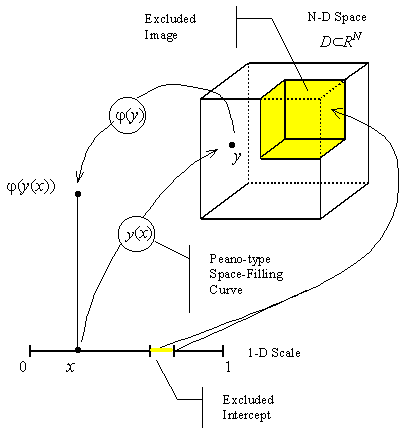
\includegraphics[scale=1.9]{images/peano1.png}
              \end{figure}
            \end{minipage}
            \end{block}
        \end{column}
        \begin{column}[t]{0.48\paperwidth}
          \begin{block}{Способ распараллеливания}

          \end{block}
            \begin{block}{Результаты}
            \end{block}
        \end{column}
    \end{columns}
\end{frame}
\end{document}
